\section{Confusion Matrices} \label{sec:res/confusion}

The following subsections will present a visualization of the predictions made by the two best models for every label group in table \ref{tab:res/performance}. Visualizations are plotted from the confusion matrices from which the classification accuracies were calculated. Therefore, the following visualizations will display one row and one column for every class in a label group. Each input sequence is passed through the model and added to one cell, whose row and column correspond to its correct and predicted class. The counts in every cell are finally normalized for every row (true class). The resulting values in each cell can therefore be interpreted as the "probability that the model will predict [column class] given [row class] input." A perfect classification model will only have one's along the diagonal. Off-diagonal values represent misclassifications.

\newpage
\subsection{State Label Groups}

% \begin{figure}[h]
%     \begin{subfigure}[b]{1\textwidth}
%         \centering
%         \includegraphics[width=\textwidth]{figures/res_B_FCN_fstate.png}
%         \caption{Best model: \acrlong{fcn}}
%         \label{fig:res/conf_fstate_B}
%     \end{subfigure}
%     \begin{subfigure}[b]{1\textwidth}
%         \centering
%         \includegraphics[width=\textwidth]{figures/res_NB_ResNet11_fstate.png}
%         \caption{Next-best model: \acrlong{resnet11}}
%         \label{fig:res/conf_fstate_NB}
%     \end{subfigure}
%     \caption{Confusion matrices for the full state label group detailed in section \ref{sec:impl/dataset}. Cell values and color gradients indicate proportion of input segments classified as [column], with true class [row].}
% \end{figure}
\begin{figure}[h]
    \begin{subfigure}[b]{0.471\textwidth}
        \centering
        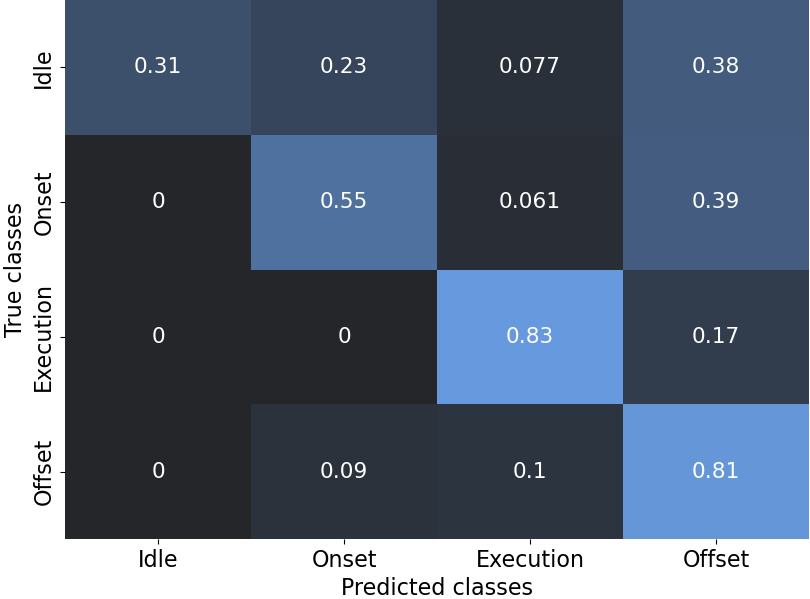
\includegraphics[width=\textwidth]{figures/res_FCN_fstate_cm.png}
        \caption{\acrshort{fs}: \acrlong{fcn}}
        \label{fig:res/conf_fstate}
    \end{subfigure}
    \begin{subfigure}[b]{0.529\textwidth}
        \centering
        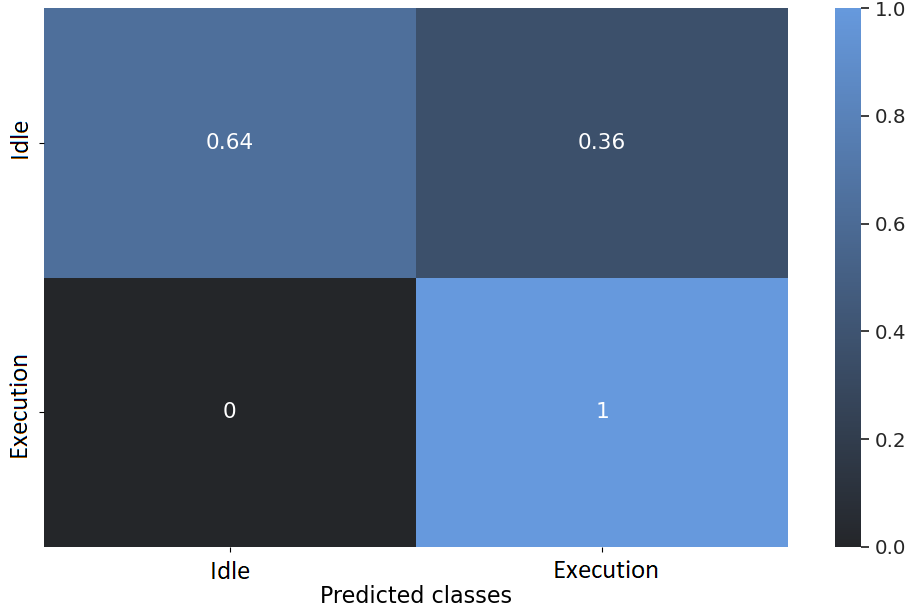
\includegraphics[width=\textwidth]{figures/res_ResNet11_bstate_cm.png}
        \caption{\acrshort{bs}: \acrlong{resnet11}}
        \label{fig:res/conf_bstate}
    \end{subfigure}
    \caption{Confusion matrices for thestate label groups detailed in section \ref{sec:impl/dataset}. Cell values and color gradients indicate proportion of input segments classified as [column], with true class [row].}
    \label{fig:res/conf_state}
\end{figure}
\FloatBarrier

% \subsection{Binary State Label Group}

% \begin{figure}[h]
%     \begin{subfigure}[b]{0.483\textwidth}
%         \centering
%         \includegraphics[width=\textwidth]{figures/res_B_ResNet11_bstate_cr.png}
%         \caption{Best: \acrlong{resnet11}}
%         \label{fig:res/conf_bstate_B}
%     \end{subfigure}
%     \begin{subfigure}[b]{0.517\textwidth}
%         \centering
%         \includegraphics[width=\textwidth]{figures/res_NB_ResNet18_bstate_cr.png}
%         \caption{Next best: \acrlong{resnet18}}
%         \label{fig:res/conf_bstate_NB}
%     \end{subfigure}
%     \caption{Confusion matrices for the binary state label group detailed in section \ref{sec:impl/dataset}. Cell values and color gradients indicate proportion of input segments classified as [column], with true class [row].}
%     \label{fig:res/conf_bstate}
% \end{figure}
% \FloatBarrier

% \newpage
\subsection{Level Label Groups}

\begin{figure}[h]
    \begin{subfigure}[b]{0.471\textwidth}
        \centering
        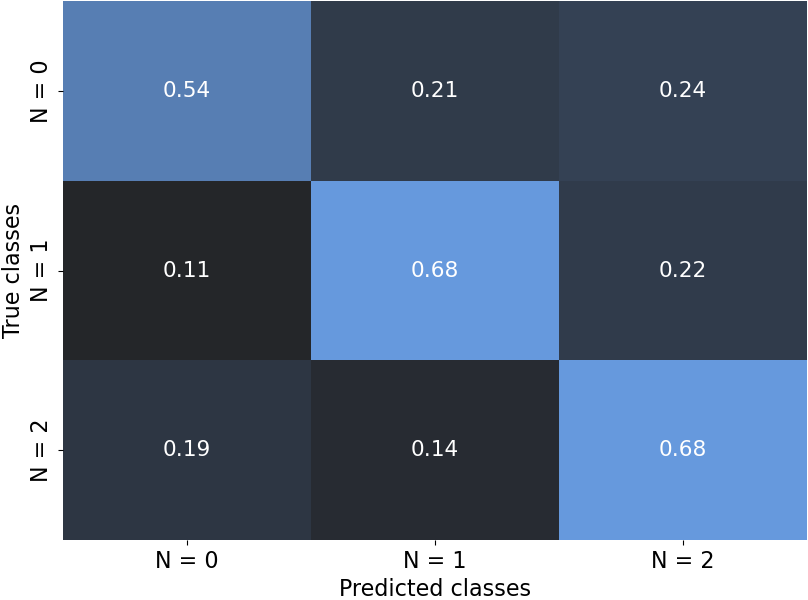
\includegraphics[width=\textwidth]{figures/res_FCN_flevel_cm.png}
        \caption{\acrshort{fl}: \acrlong{fcn}}
        \label{fig:res/conf_flevel}
    \end{subfigure}
    \begin{subfigure}[b]{0.529\textwidth}
        \centering
        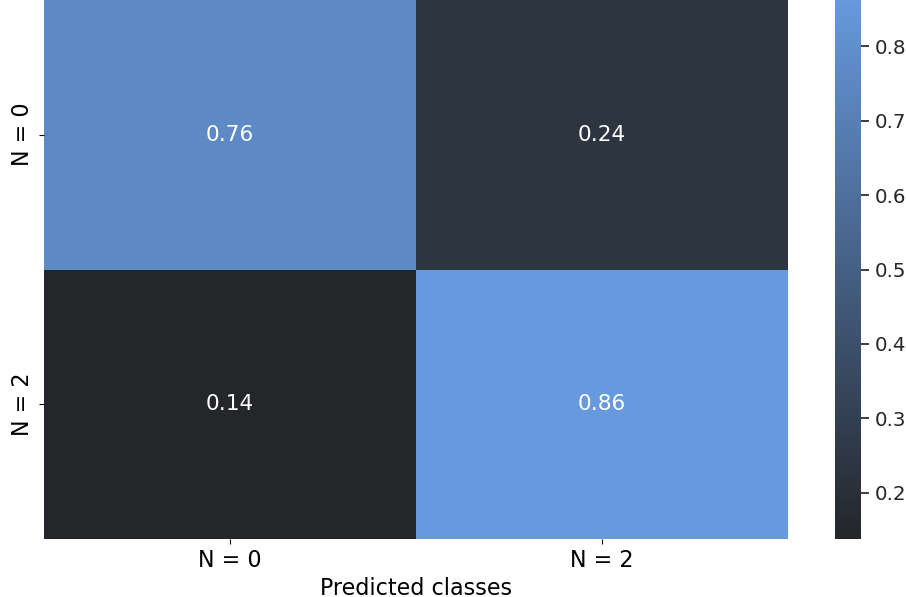
\includegraphics[width=\textwidth]{figures/res_ResNet18_blevel_cm.png}
        \caption{\acrshort{bl}: \acrlong{resnet18}}
        \label{fig:res/conf_blevel}
    \end{subfigure}
    \caption{Confusion matrices for the level label groups detailed in section \ref{sec:impl/dataset}. Cell values and color gradients indicate proportion of input segments classified as [column], with true class [row].}
    \label{fig:res/conf_level}
\end{figure}
\FloatBarrier


% \subsection{Binary Level Label Group}

% \begin{figure}[h]
%     \begin{subfigure}[b]{0.483\textwidth}
%         \centering
%         \includegraphics[width=\textwidth]{figures/res_B_ResNet18_blevel_cr.png}
%         \caption{Best: \acrlong{resnet18}}
%         \label{fig:res/conf_blevel_B}
%     \end{subfigure}
%     \begin{subfigure}[b]{0.517\textwidth}
%         \centering
%         \includegraphics[width=\textwidth]{figures/res_NB_ResNet11_blevel_cr.png}
%         \caption{Next best: \acrlong{resnet11}}
%         \label{fig:res/conf_blevel_NB}
%     \end{subfigure}
%     \caption{Confusion matrices for the binary level label group detailed in section \ref{sec:impl/dataset}. Cell values and color gradients indicate proportion of input segments classified as [column], with true class [row].}
%     \label{fig:res/conf_blevel}
% \end{figure}
% \FloatBarrier